\addcontentsline{toc}{section}{\protect\numberline{}Einleitung}
\section*{Einleitung}
Regelungstechnik Labor ist eine Blockwoche, welche an der Hochschule Luzern - 
Technik \& Architektur angeboten wird. Dies sind meine persönlichen Lösungen 
zur Vorbereitungsübung. Die \begin{aufgabe}Aufgabenteile\end{aufgabe} ~sind 
jeweils \begin{aufgabe}markiert\end{aufgabe}. Diese markierten Teile und 
\autoref{fig:aufgabe} stammen aus der Vorbereitungsübung vom 
Modulverantwortlichen Thierry Prud'homme. \\
Diese sind auch digital unter \url{https://github.com/daniw/rt-l} abrufbar. 
\\
\subsubsection*{Aufgabe}
\begin{aufgabe}
    In \autoref{fig:aufgabe} ist ein einfacher Antrieb mit einem 
    Gleichstrommotor zu sehen. Es wird versucht die Drehzahl $\omega(t)$ zu 
    regeln.
    \begin{figure}[h!]
        \centering
        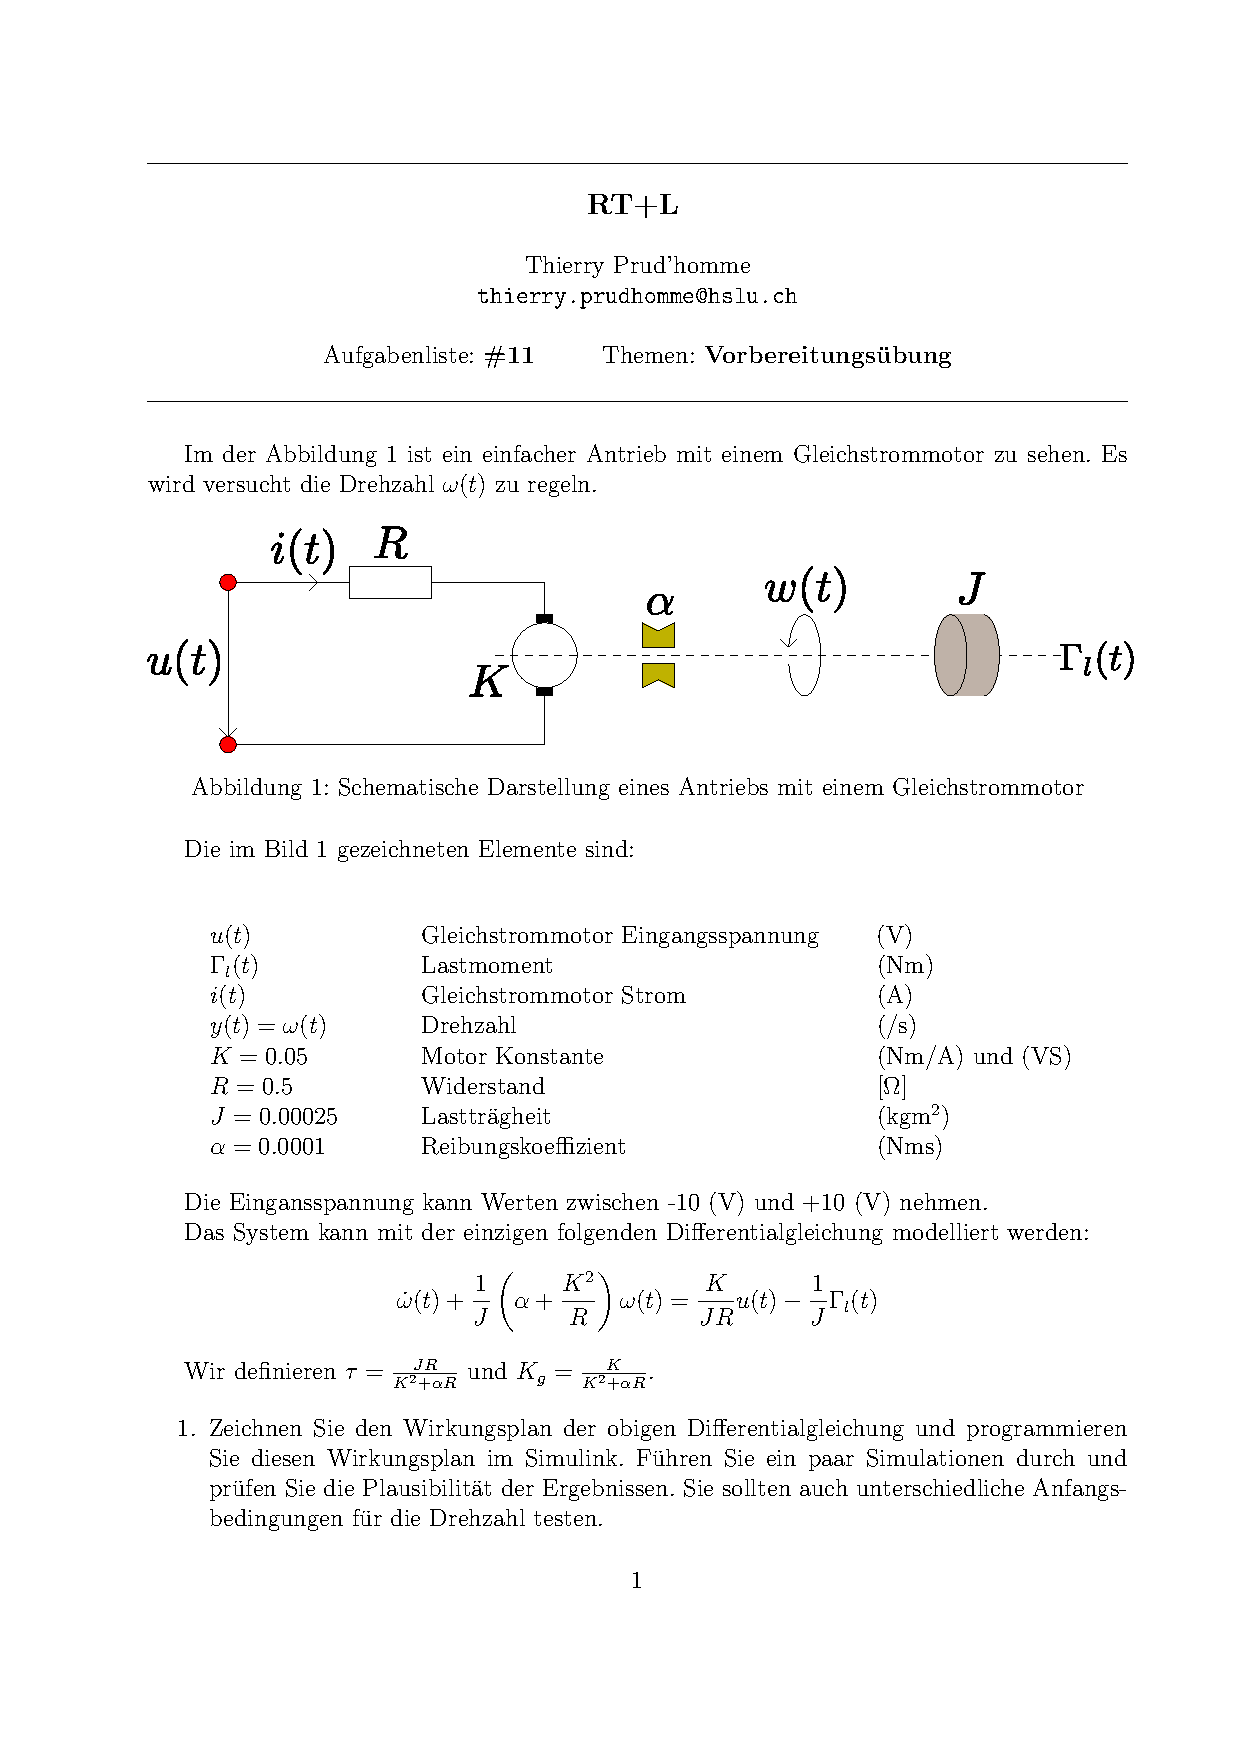
\includegraphics[page=1, width=0.7\textwidth, trim=70 470 50 250, clip=true]
            {aufgabe/RTL_VorbereitungUebung.pdf}
        \caption{Schematische Darstellung eines Antriebs mit einem Gleichstrommotor}
        \label{fig:aufgabe}
    \end{figure}
    \\
    Die in \autoref{fig:aufgabe} gezeichneten Elemente sind: \\
    \begin{tabular}{@{}lll}
        $u(t)$              & Gleichstrommotor Eingangsspannung & [V] \\
        $\Gamma_l(t)$       & Lastmoment                        & [Nm] \\
        $i(t)$              & Gleichstrommotor Strom            & [A] \\
        $y(t) = \omega(t)$  & Drehzahl                          & [1/s] \\
        $K = 0.05$          & Motor Konstante                   & [Nm/A] und [VS] \\
        $R = 0.5$           & Widerstand                        & [$\Omega$] \\
        $J = 0.00025$       & Lastträgheit                      & [kgm$^2$] \\
        $\alpha = 0.0001$   & Reibungskoeffizient               & [Nms] \\
    \end{tabular}
    \\
    Die Eingansspannung kann Werte zwischen -10 [V] und +10 [V] einnehmen. \\
    Das System kann mit der folgenden Differentialgleichung modelliert werden:
    \[ \dot{\omega}(t) 
        + \frac{1}{J} \cdot \left(\alpha + \frac{K^2}{R}\right) \cdot \omega(t) 
        = \frac{K}{J \cdot R} \cdot u(t) - \frac{1}{J} \cdot \Gamma_l(t)
    \]
    Wir definieren $\frac{J \cdot R}{K^2 + \alpha \cdot R}$ und 
    $K_g = \frac{K}{K^2 + \alpha \cdot R}$. 
\end{aufgabe}
